\chapter{Cauchy-Schwarz不等式\\及其证明}

\section{定理描述}

\subsection*{一般形式}

Cauchy-Schwarz不等式的一般描述如下
\begin{theorem}
    已知$a_1,\cdots,a_n,b_1\cdots,b_n$是实数,则
    \begin{equation}
        (\sum\limits_{i=1}^{n}a_ib_i)^2\leqslant (\sum\limits_{i=1}^{n}a^2_i)(\sum\limits_{i=1}^{n}b^2_i) 
    \end{equation}

    等号成立的充分必要条件是
    \begin{equation}
        a_i=\lambda b_i,\ \ i=1,\cdots n
    \end{equation}
\end{theorem}

\subsection*{推广到复数形式}
不等式可以推广到复数。如何推广呢?不等式只有在实数时才有意义,对于复数则需要考虑角度和模长
大小关系。

\begin{theorem}
    已知$a_1,\cdots,a_n,b_1\cdots,b_n$是复数,则
    \begin{equation}
        |\sum\limits_{i=1}^{n}a_ib_i|^2\leqslant (\sum\limits_{i=1}^{n}|a_i|^2)(\sum\limits_{i=1}^{n}|b_i|^2) 
    \end{equation}

    等号成立的充分必要条件是
    \begin{equation}
        a_i=\lambda b_i,\ \ i=1,\cdots n
    \end{equation}
\end{theorem}

\subsection*{矩阵形式}

根据线性代数的理论:\textsl{任意正定对称矩阵都可以定义内积}。因此若$A=a_{ij}$为正定对称矩阵,则
$Cauchy$不等式存在
\begin{theorem}
    已知$(a_{ij})_{kl}$是正定对称矩阵,对于$x_1,\cdots,x_n,y_1.\cdots,y_n$是任意复数或者实数,则
    \begin{equation}
        |\sum\limits_{i=1}^{n}a_{ij}x_iy_j|\leqslant \sqrt{\sum\limits_{i,j=1}^{n}a_{ij}x_ix_j}
        \sqrt{\sum\limits_{i,j=1}^{n}a_{ij}y_iy_j}
    \end{equation}

    等号成立的充分必要条件是
    \begin{equation}
        a_i=\lambda b_i,\ \ i=1,\cdots n
    \end{equation}
\end{theorem}

\subsection*{无穷级数形式}

\begin{theorem}
    已知$a_1,\cdots,a_n,\cdots,b_1\cdots,b_n,\cdots$是复数,则
    \begin{equation}
        |\sum\limits_{i=1}^{\infty}a_ib_i|\leqslant 
        (\sum\limits_{i=1}^{\infty}|a_i|^2)^{\frac{1}{2}}
        (\sum\limits_{i=1}^{\infty}|b_i|^2)^{\frac{1}{2}}
    \end{equation}

    等号成立的充分必要条件是
    \begin{equation}
        a_i=\lambda b_i,\ \ i=1,\cdots ;\ \ \lambda\in \mathbb{C}
    \end{equation}
    \begin{equation}
        \sum\limits_{i=1}^{\infty}|a_i|^2<\infty
    \end{equation}
    \begin{equation}
        \sum\limits_{i=1}^{\infty}|b_i|^2<\infty
    \end{equation}
\end{theorem}

\subsection*{积分形式}

\begin{theorem}
    已知$f,g$是区间$[a,b]$上的连续函数,$f,g\in C[a,b]$,则
    \begin{equation}
        |\int_{a}^{b}f(x)g(x)dx|^2\leqslant \int_{a}^{b}|f(x)|^2dx \int_{a}^{b}|g(x)|^2dx 
    \end{equation}
\end{theorem}

\subsection*{$H\ddot{o}lder$不等式}
\begin{theorem}
    已知$a_1,\cdots,a_n,b_1\cdots,b_n$是复数,$p,q\geqslant 1$,$\frac{1}{p}+\frac{1}{q}=1$,则
    \begin{equation}
        |\sum\limits_{i=1}^{n}a_ib_i|\leqslant (\sum\limits_{i=1}^{n}|a_i|^p)^{\frac{1}{p}}
        (\sum\limits_{i=1}^{n}|b_i|^q)^{\frac{1}{q}} 
    \end{equation}
\end{theorem}

\subsection*{广义Cauchy-Schwarz不等式}

\begin{theorem}
    一般$n$维向量空间中的Cauchy-Schwarz不等式形式为
    \begin{equation}
        |a\cdot b|\leqslant \Vert a\Vert \Vert b\Vert
    \end{equation}
\end{theorem}

\section{余弦定律}
考虑三角形$\bigtriangleup ABC$,三条边的分量分别是
\begin{equation}
    \overrightarrow{a}=\overrightarrow{AB},\overrightarrow{b}=\overrightarrow{AC},
    \overrightarrow{c}=\overrightarrow{CB}=\vec{a}-\vec{b}
\end{equation}

\begin{figure}[H]
    \centering
    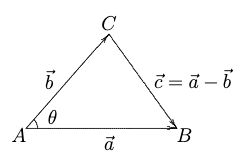
\includegraphics[scale=0.6]{figures/余弦定律.png}
    \caption{余弦定律}
\end{figure}

根据余弦定律$|\vec{a}|^2+|\vec{b}|^2-|\vec{a}-\vec{b}|^2=2|\vec{a}||\vec{b}|\cos{\theta}$以及余弦的性质$|\cos{\theta}|\leqslant 1$,可得
\begin{equation}
    |\vec{a}\cdot\vec{b}|\leqslant |\vec{a}||\vec{b}|
\end{equation}

这就是Cauchy-Schwarz不等式。他告诉我们Cauchy-Schwarz不等式的几何意义:三角形两边的内积小于两个向量长度的乘积。

\section{证明}

考虑$b$在$a$上的投影之差的最短距离,设
\begin{equation}
    \overrightarrow{c}=\vec{b}-\lambda \vec{a},\ \ \ \ \lambda\in \mathbb{R}
\end{equation}

$\vec{c}$的长度

\begin{eqnarray}
    |\vec{c}|^2=\vec{c}\cdot \vec{c}=|\vec{a}|^2\lambda^2+2\vec{a}\cdot \vec{b}\lambda +|b|^2>0
\end{eqnarray}

上式可视为$\lambda$的二次方程,且与$\lambda$轴没有交点

\begin{equation}
    \bigtriangleup = (2\vec{a}\vec{b})^2-4|\vec{a}|^2|\vec{b}|^2\leqslant 0
\end{equation}

因此有
\begin{equation}
    |\vec{a}\cdot \vec{b}|\leqslant |\vec{a}||\vec{b}|
\end{equation}